\documentclass[conference]{IEEEtran}
\IEEEoverridecommandlockouts
% The preceding line is only needed to identify funding in the first footnote. If that is unneeded, please comment it out.
\usepackage{cite}
\usepackage{amsmath,amssymb,amsfonts}
\usepackage{algorithmic}
\usepackage{graphicx}
\usepackage{textcomp}
\usepackage{xcolor}
\def\BibTeX{{\rm B\kern-.05em{\sc i\kern-.025em b}\kern-.08em
    T\kern-.1667em\lower.7ex\hbox{E}\kern-.125emX}}
\begin{document}

\title{Implementation of a Two's Complement Circuit*\\
{\footnotesize \textsuperscript{*}Note: Project of the course ICE3405P-Computer Organization}
}

\author{\IEEEauthorblockN{Nan Lin}
\IEEEauthorblockA{\textit{SPEIT} \\
\textit{Shanghai Jiao Tong University}\\
Shanghai, China \\
lns\_brandon@sjtu.edu.cn}
\and
\IEEEauthorblockN{Yanxu Meng}
\IEEEauthorblockA{\textit{SPEIT} \\
\textit{Shanghai Jiao Tong University}\\
Shanghai, China \\
email address or ORCID}
}

\maketitle

\begin{abstract}
This document is a model and instructions for \LaTeX.
This and the IEEEtran.cls file define the components of your paper [title, text, heads, etc.]. *CRITICAL: Do Not Use Symbols, Special Characters, Footnotes, 
or Math in Paper Title or Abstract.
\end{abstract}

\begin{IEEEkeywords}
component, formatting, style, styling, insert
\end{IEEEkeywords}


\section{Question 1-5}

\subsection{Question 1}\label{sec:q_A}

The two's complement of a binary number is obtained by following the rule:
\begin{itemize}
    \item If the sign bit (highest bit) is 0, it indicates that the sign-magnitude representation is a positive number. In this case, the binary number is unchanged.
    \item If the sign bit is 1, we should invert its digits and add one to the least significant bit. 
\end{itemize}

This method allows for binary arithmetic and simplifies the design of digital circuits for arithmetic operations.
A straightforward implementation is to adopt different operation modes depending on the sign bit using a multiplexer. A typical multiplexer is shown in Figure~\ref{fig:multiplexer}. For an 8-bit binary number, suppose that it could be represented as:
\begin{equation}
    \overline{s_7 s_6 s_5 s_4 s_3 s_2 s_1 s_0}
\end{equation}

$s_7$ is the sign bit, therefore playing the role of Select for all other bits ($s_0$ to $s_6$) here.

\begin{figure}[h!]
    \centering
    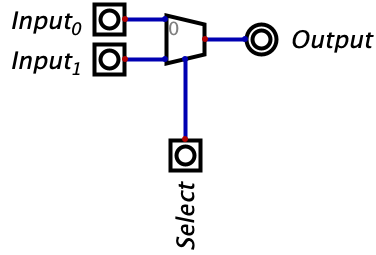
\includegraphics[width=0.3\textwidth]{assets/multiplexer.png}
    \caption{A Multiplexer. When Select is 0, the output corresponds to the value of $\text{Input}_0$, neglecting the condition of $\text{Input}_1$. Inversely, when Select is 1, the output corresponds to the value of $\text{Input}_1$.}
    \label{fig:multiplexer}
\end{figure}

In order to add one to the least significant bit, an adder is required.
A half-adder is a fundamental component in digital arithmetic. It takes two single-bit binary inputs and produces a sum and carry output. The truth table for a half-adder is shown below:

\begin{table}[h!]
\centering
\begin{tabular}{|c|c|c|c|}
\hline
A & B & Sum (Result) & CarryOut \\ \hline
0 & 0 &  0  &   0   \\ \hline
0 & 1 &  1  &   0   \\ \hline
1 & 0 &  1  &   0   \\ \hline
1 & 1 &  0  &   1   \\ \hline
\end{tabular}
\caption{Truth table for a half-adder}
\end{table}

The corresponding half-adder circuit diagram is illustrated in Figure~\ref{fig:half_adder}.

\begin{figure}[h!]
\centering
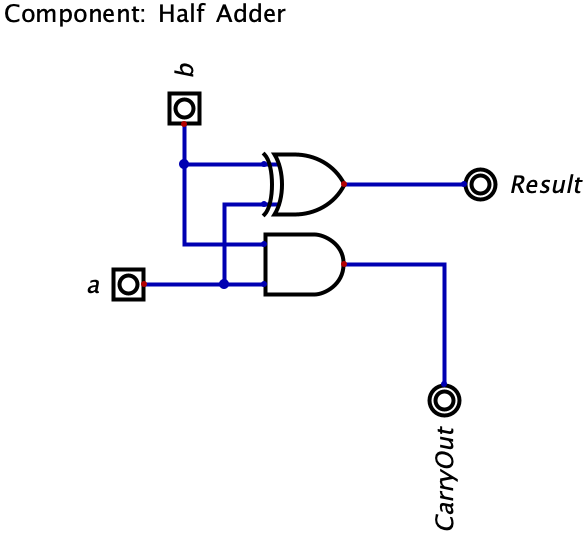
\includegraphics[width=0.4\textwidth]{assets/half_adder.png}
\caption{Half-Adder Circuit}
\label{fig:half_adder}
\end{figure}

We use a half-adder rather than a full adder for multiple reasons:
\begin{itemize}
    \item A half-adder has a relatively simpler structure. Most importantly, its depth is one less than a full adder and it contains fewer gates which provides the advantage of lower energy consumption and less time consumption.
    \item A half-adder is proved to be effective because to implement a two's complement circuit, we only need to calculate $\overline{s_6 \dots s_0} + \overline{0 \dots 01}$ (taking 8-bit binary numbers as an example). Since all the 
    bits are 0, we can put the CarryOut onto the place of another adder.
\end{itemize}

To implement an 8-bit two's complement circuit, we combine multiple half-adders; each half-adder is used to calculate the corresponding bit of the binary number. The process involves inverting each bit of the input number and then adding one using a series of adders. The detailed circuit diagram is shown in Figure~\ref{fig:twos_complement}.



\begin{figure}[h!]
\centering
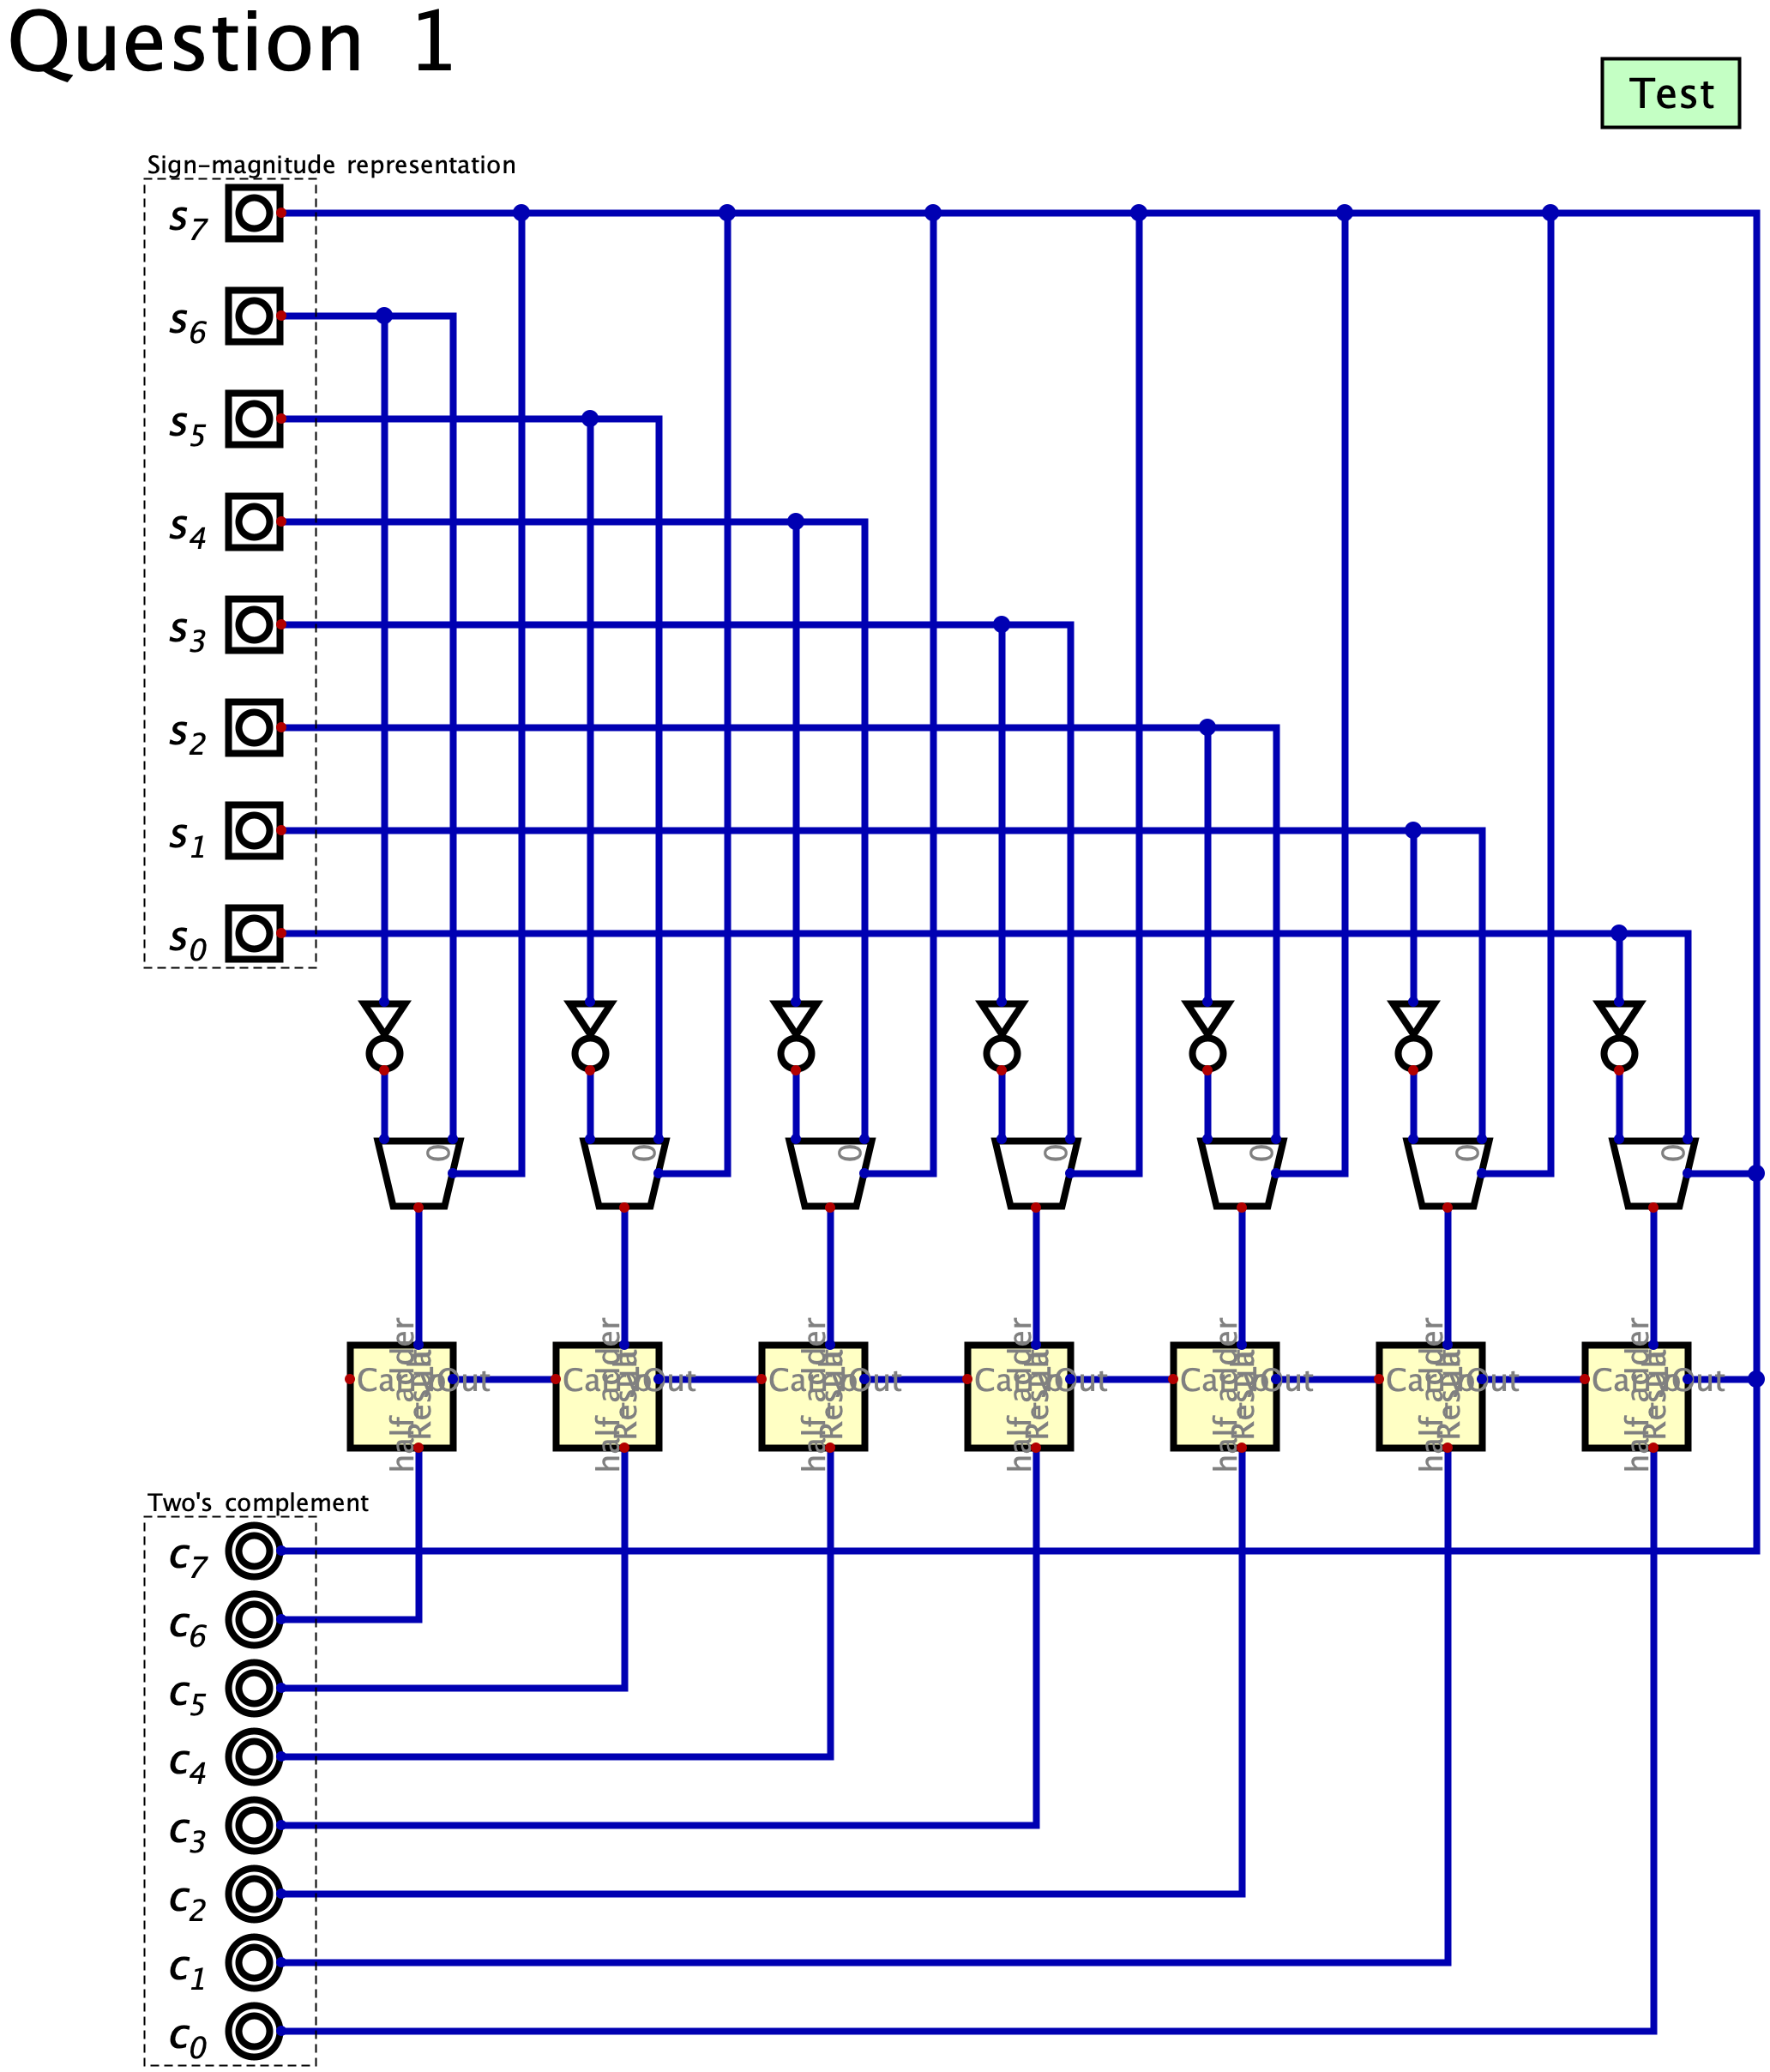
\includegraphics[width=0.45\textwidth]{assets/twos_complement.png}
\caption{8-bit Two's Complement Circuit. The yellow box is a half-adder implemented in Figure~\ref{fig:half_adder}}
\label{fig:twos_complement}
\end{figure}


\subsection{Question 2}

To analyze the depth and complexity of the two's complement circuit for 8 bits, we divide the process into two stages.

The first stage is the \textbf{inversion stage}. Each bit requires a NOT gate, thus in the first stage:
\begin{itemize}
\item Depth: 1 (because all of the NOT gates operate simultaneously)
\item Complexity: 7 (NOT gates)
\end{itemize}

The second stage is the \textbf{addition stage}. For each bit, a half-adder is applied.
The depth of each half-adder is 1 and the complexity is 2. Since there are 7 bits that need to be calculated one by one, in the second stage:
\begin{itemize}
    \item Depth: $7 \times 1 = 7$
    \item Complexity: $7 \times 2 = 14$
\end{itemize}

Summing up the two stages, the depth of calculation of the two's complement of an 8-bit binary number is $1 + 7 = 8$ and the complexity is $7 + 14 = 21$.

We expand the results to any $2^p$-bit ($p \in \mathbb{N}$) two's complement circuit.

\begin{enumerate}
\item In the \textbf{inversion stage}, the depth is 1 due to parallelization, and the complexity is $2^p - 1$.
\item In the \textbf{addition stage}, the depth is $2^p - 1$ and the number of gates required is $2 \times (2^p - 1)$.
\end{enumerate}

\textbf{
Conclusion: For a $2^p$-bit two's complement circuit, the depth is $2^p$, and the complexity is $3(2^p - 1)$.
}

\subsection{Question 3}

In order to reduce the depth of the circuit, having a closer look at the circuit implemented in Section~\ref{sec:q_A}, the main problem is that the CarryOut is passed on in series.
In other words, to calculate the two's representation of $s_k$ of a $2^p$-bit binary number ($0 < k \leq 2^p-2$), we have to wait for the values of $k-1$ CarryOuts one by one.

To optimize this process, we propose a new version of the two's complement circuit for an 8-bit machine by employing a method that uses two 4-bit lookahead carry adders in series. This approach allows for the calculation of four bits and their carry at once, then passing the carry to the next set of four bits. This reflects the divide and conquer strategy.

The implementation involves the following steps:
\begin{enumerate}
    \item \textbf{Inversion Stage}: This stage is unchanged, where each of the 8 bits is inverted using NOT gates.
    \item \textbf{Addition Stage}: The 8-bit addition is divided into two 4-bit additions using lookahead carry adders.
    \begin{itemize}
        \item \textbf{First 4-bit Adder}: Computes the result and the carry for the first four bits.
        \item \textbf{Second 4-bit Adder}: Computes the result for the next three (but not four!) bits.
    \end{itemize}
\end{enumerate}

We then implement a classical 4-bit lookahead carry adders which could be found in textbooks. First we introduce two fundamental components.

In digital circuits, the Generate-Propagate (GP) logic is used to speed up the carry calculation in adders. For two binary inputs $A_i$ and $B_i$, the generate ($G_i$) and propagate ($P_i$) signals are defined as:
\begin{equation}
g_i = a_i \cdot b_i
\end{equation}
\begin{equation}
p_i = a_i + b_i
\end{equation}
The GP generator is used to generate respectively the AND and OR result of two variables, this result will be deploited later on.
The implementation of the GP generator is displayed in Figure~\ref{fig:gp_generator}. For any bit, the value is 
\begin{equation}
    \forall k \in [\![1, 2^p-2]\!], \quad s_k = a_k + b_k + c_{k-1}
\end{equation}
where $c_{k-1}$ is the carry bit into position $k$.

\begin{figure}[h!]
\centering
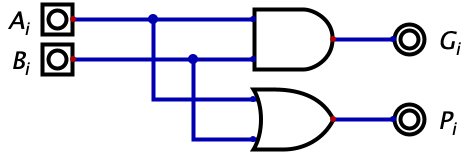
\includegraphics[width=0.4\textwidth]{assets/generate_gp.png}
\caption{GP Generator Circuit}
\label{fig:gp_generator}
\end{figure}

The carry bits could be calculated as follows:

\begin{equation}\label{eq:carry-bit}
    c_{i+1} = a_i b_i + (a_i + b_i) c_i
\end{equation}

owing to the reason that the carry bit is 1 if

\begin{itemize}
    \item Both of the two bits are $1$
    \item Any of the two bits is $1$ and the carry bit from the former bit is 1.
\end{itemize}

Here we replace $a_ib_i$ and $a_i + b_i$ with $g_i$ and $p_i$. The Equation~\ref{eq:carry-bit} turns into:

\begin{equation}\label{eq:carry-bit-deduction}
    c_{i+1} = g_i + p_i c_i
\end{equation}

We therefore deduce all the carry bits based on Equation~\ref{eq:carry-bit-deduction}:
\begin{align}
    c_1 &= g_0 + p_0 c_0 \label{eq:temp1}\\
    c_2 &= g_1 + p_1 c_1 = g_1 + p_1 g_0 + p_1 p_0 c_0 \\
    c_3 &= g_2 + p_2 c_2 = g_2 + p_2 g_1 + p_2 p_1 g_0 + p_2 p_1 p_0 c_0 \\
    c_4 &= g_3 + p_3 c_3 = g_3 + p_3 p_2 g_1 + p_3 p_2 p_1 g_0 + p_3 p_2 p_1 p_0 c_0 \label{eq:temp2}
\end{align}




A full adder also takes the CarryIn of the formal bit compared to a half adder. It is displayed in Figure~\ref{fig:full_adder}. 


\begin{figure}[h!]
    \centering
    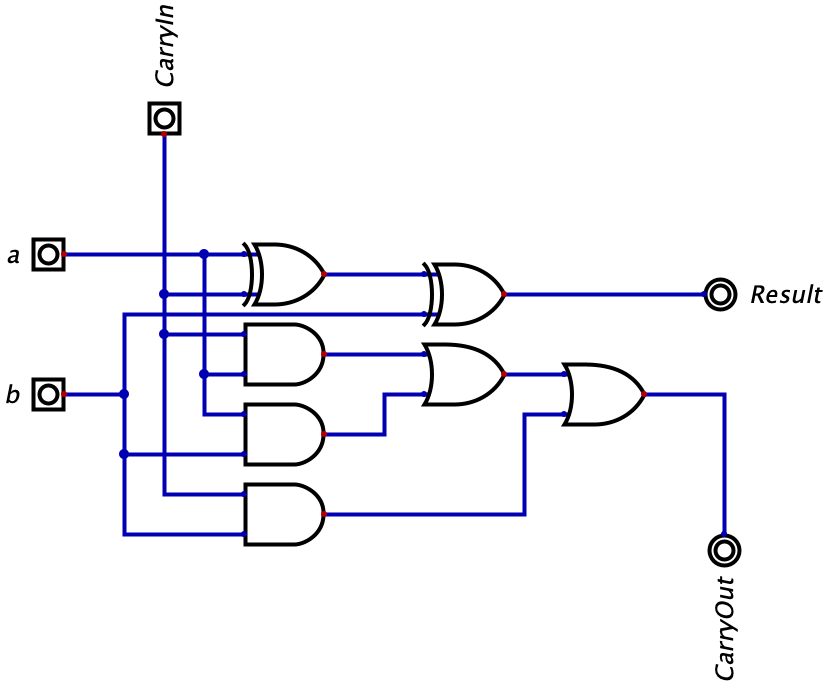
\includegraphics[width=0.5\textwidth]{assets/full_adder.png}
    \caption{Full-Adder Circuit}
    \label{fig:full_adder}
\end{figure}

A classic 4-bit lookahead carry adder based on full-adders is shown in Figure~\ref{fig:lca}. We then combine the two 4-bit adder in series. The final two's complement circuit is shown in Figure~\ref{fig:tc-dq}. When the
sign bit is 1, it implies that we should invert its digits and add one to the least significant bit. In this case, the sign bit is passed to the first CarryIn input, and the operation of the full adder is identical to:
\begin{align}\label{eq:carry-bits-result}
    \overline{a_3 a_2 a_1 a_0} &+ \overline{0000} \quad \text{with CarryIn } 1 \\
    \overline{0 a_6 a_5 a_4} &+ \overline{0000} \quad \text{with CarryIn from the former 4-bit adder}
\end{align}

\begin{figure}[h!]
    \centering
    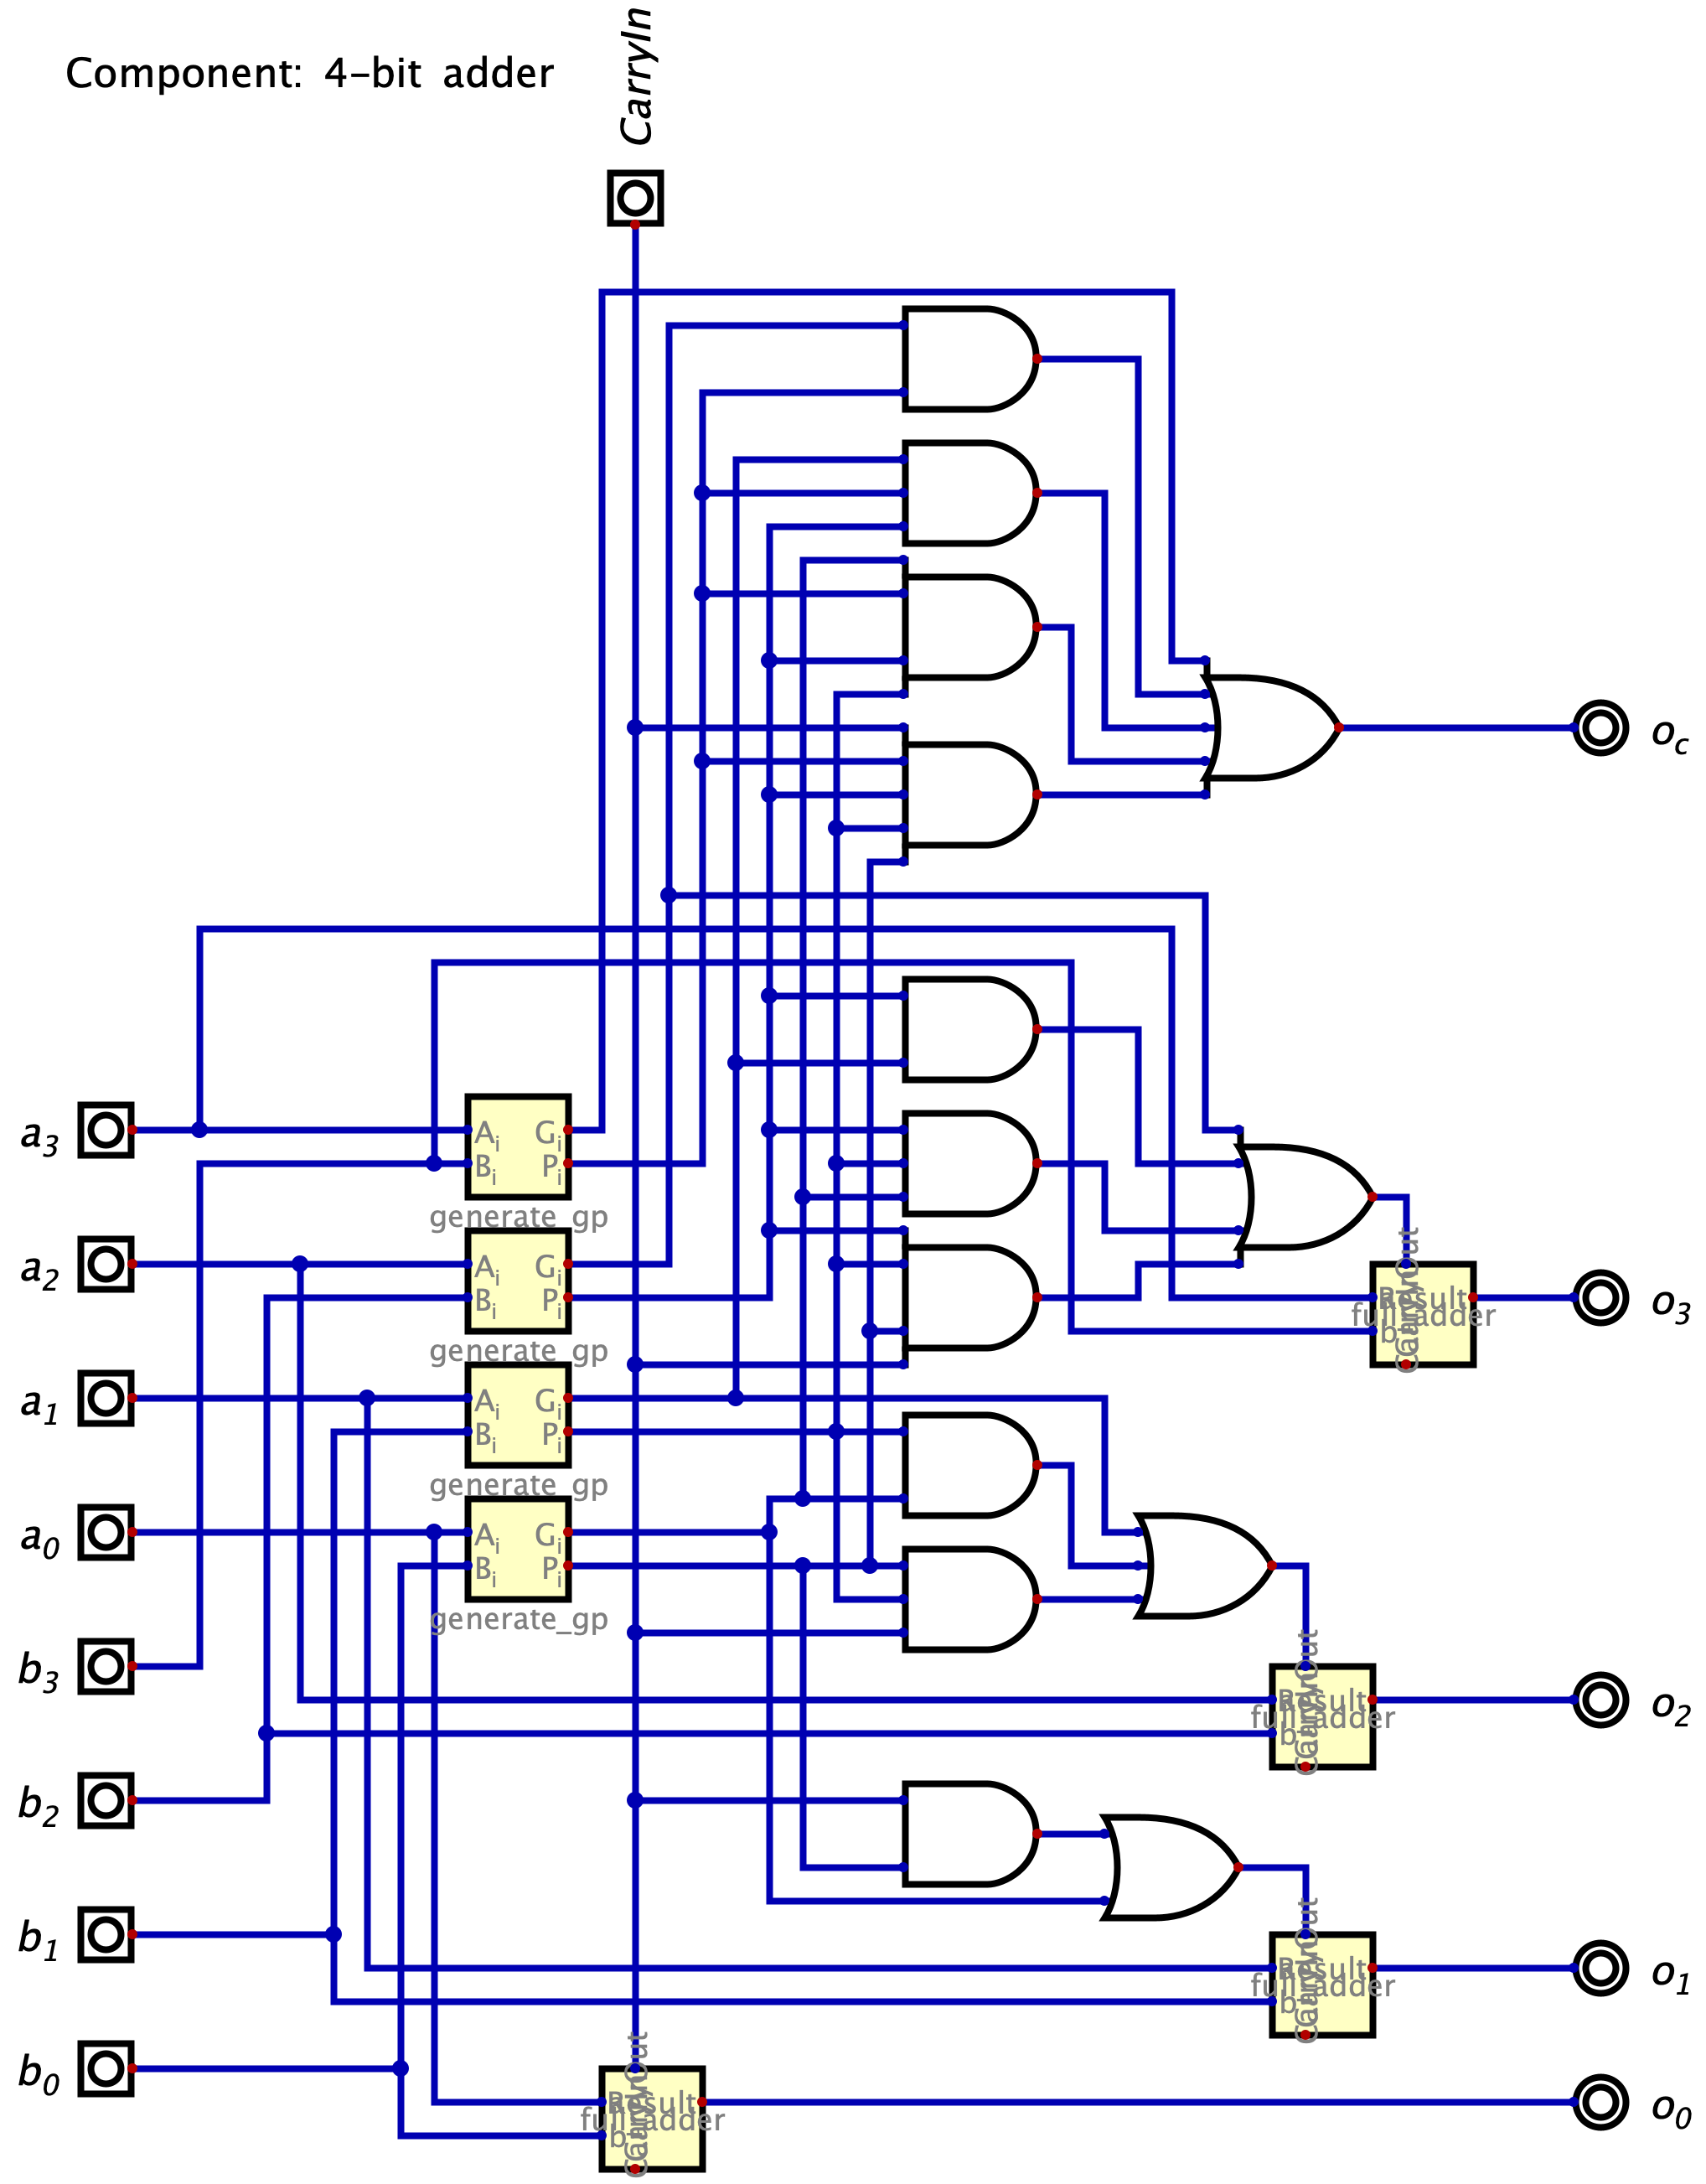
\includegraphics[width=0.5\textwidth]{assets/adder_4bits.png}
    \caption{4-bit Lookahead Carry Adder based on Full-Adders}
    \label{fig:lca}
    \end{figure}


    \begin{figure}[h!]
        \centering
        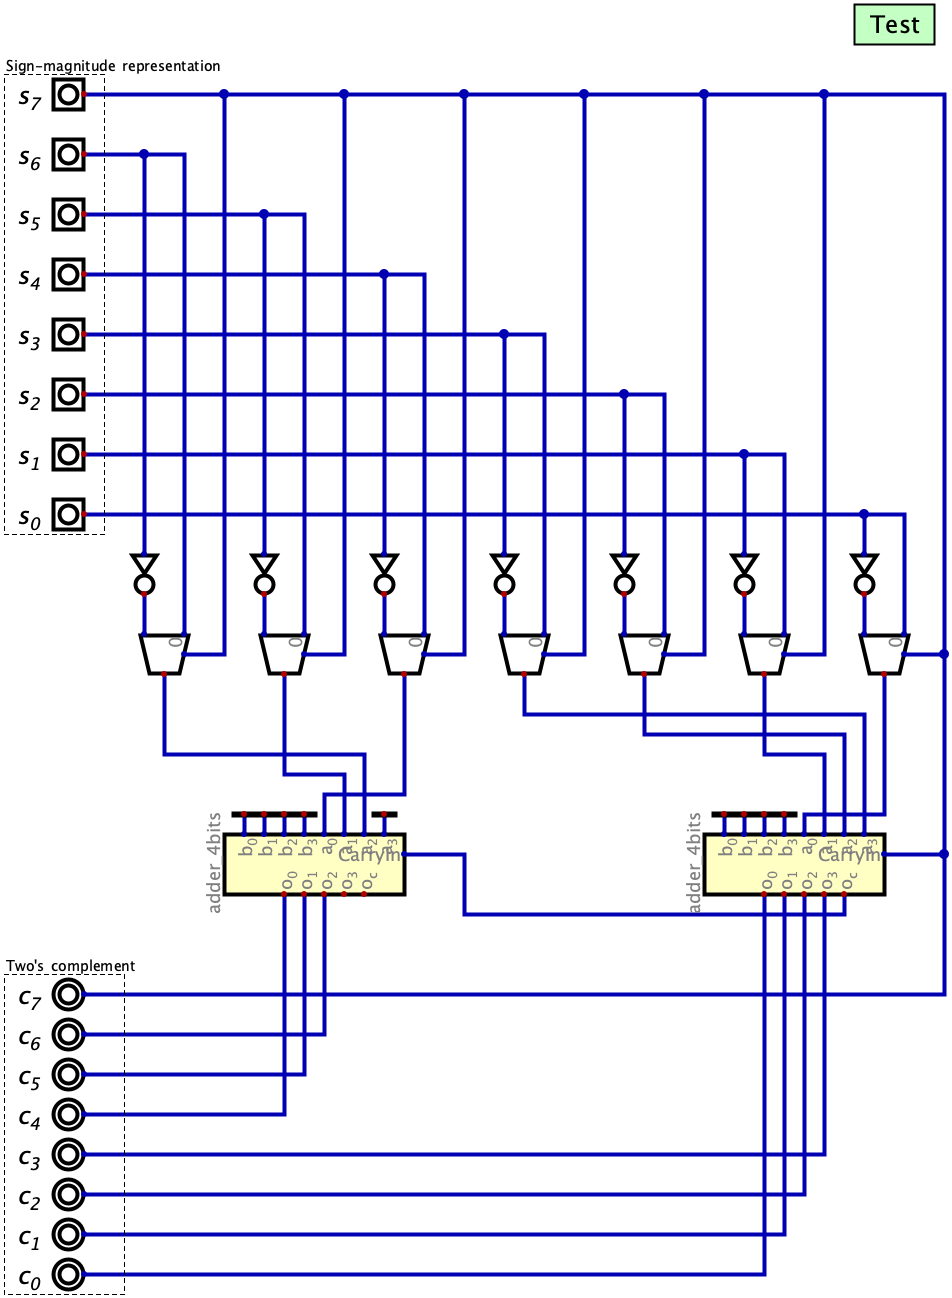
\includegraphics[width=0.45\textwidth]{assets/twos_complement_dq.png}
        \caption{8-bit Two's Complement Circuit (Divide and Conquer Method) Based on Full-Adders}
        \label{fig:tc-dq}
        \end{figure}

The reason why we put in series of 4-bit Lookahead Carry Adder instead of series of 8 (or even 16, 32, ...)-bit Lookahead Carry Adder is to reduce the complexity of designing the circuit.
As shown in Figure~{fig:lca}, to implement a 4-bit Lookahead Carry Adder, we need an AND gate with 5 inputs. This is already hard to fabricate in reality and it consume much more time and energy if we separate the AND gates.

However, there are still spaces of optimization. This indeed is the implementation of a standard additionner between two 8-bit binary numbers. Here, we're only required to perform addition on binary numbers with 1.
We could throw out 0s and full-adders and adopt half-adders.

Furthermore, since the other adder is always 0 in Equation~\ref{eq:carry-bits-result}, the G(enerate) signal is always 0. This implies for any valid value of $g_i$, they should be 0. Equations~\ref{eq:temp1} to~\ref{eq:temp2} could be transformed into:
\begin{align}
    c_1 &= p_0 c_0 \\
    c_2 &= p_1 p_0 c_0 \\
    c_3 &= p_2 p_1 p_0 c_0 \\
    c_4 &= p_3 p_2 p_1 p_0 c_0
\end{align}

Based on these two points, the 4-bit Lookahead Carry Adder could be optimized as shown in Figure~\ref{fig:lca-optimize}.


\begin{figure}[h!]
    \centering
    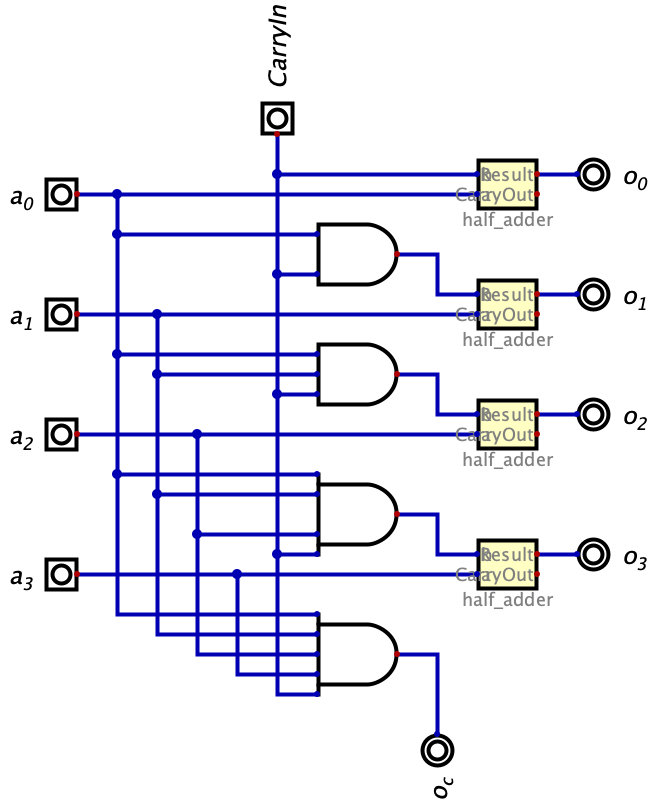
\includegraphics[width=0.45\textwidth]{assets/adder_4bits_copy.png}
    \caption{Optimized 4-bit Lookahead Carry Adder based on Half-Adders and simplified gates}
    \label{fig:lca-optimize}
    \end{figure}

The corresponding 8-bit two's complement circuit is shown in Figure~\ref{fig:tc-dq-optimize}.


\begin{figure}[h!]
    \centering
    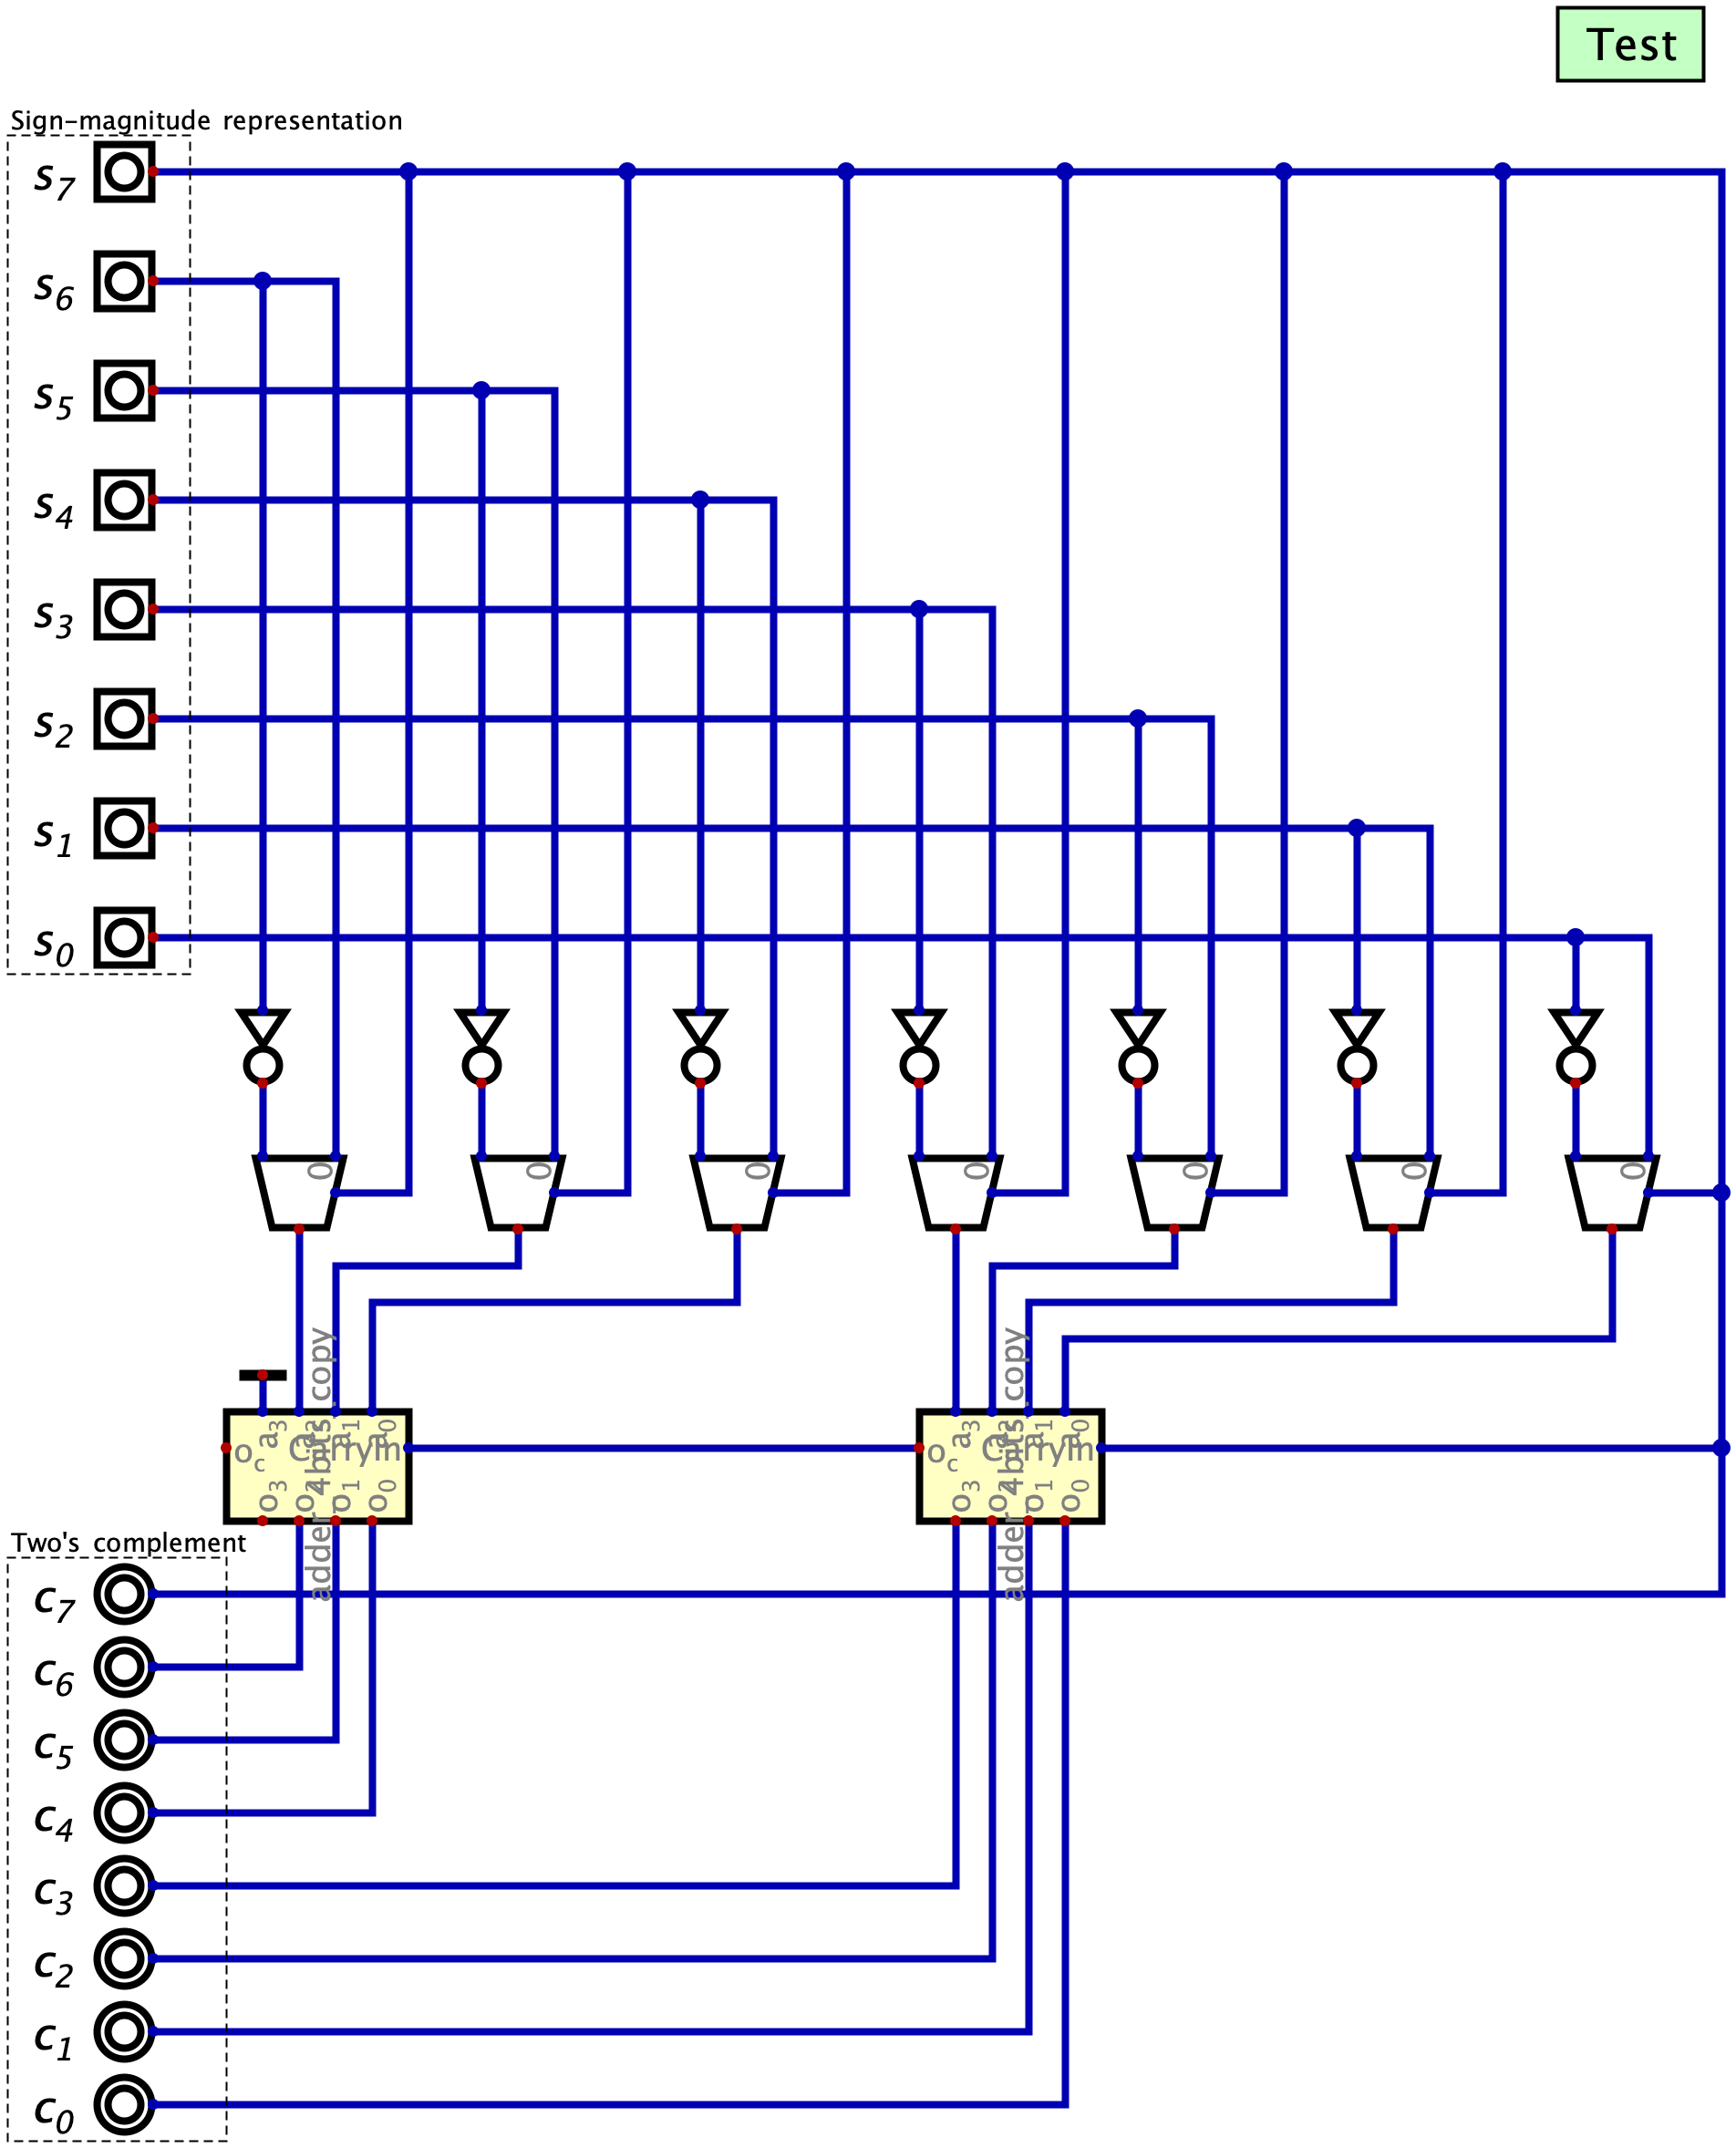
\includegraphics[width=0.45\textwidth]{assets/twos_complement_dq_copy.png}
    \caption{Optimized 8-bit Two's Complement Circuit (Divide and Conquer Method) Based on 4-bit Lookahead Carry Adder Proposed in Figure~\ref{fig:lca-optimize}}
    \label{fig:tc-dq-optimize}
    \end{figure}
    
\subsection{Question 4}

For a 8-bit two's complement circuit, to calculate the depth and complexity of the circuit, we divide the circuit into two parts:
\begin{enumerate}
    \item In the \textbf{inversion stage}, all components are inversed simultaneously, thus depth is 1 and amount of NOT gates required is 7.
    \item In the \textbf{addition stage}, the two 4-bit lookahead carry adder one after another. They are connected in series.
          For a single 4-bit lookahead, its depth is 2 since one for the AND gates and one for the Half-Adders. The number of gates utilized is:
          \begin{equation}
            4 +4 \times 2 = 12
          \end{equation}
          Since there are two lookahead carry adders, therefore, its depth is 4 and its complexity is 24.

\end{enumerate}

Therefore, for a 8-bit circuit, its depth is $1+4=5$ and its complexity is $7+24=31$.

Now, for any $2^p$-bit two's complement circuit, the inversion stage is unchanged: the depth is 1 and the complexity is $2^p-1$ in this stage. We need to count how many 4-bit Lookahead adders needed.

The main concept is to divide the large binary number into groups of 4-bit binary numbers. After that, we put them into series. The amount of groups: 
\begin{equation}
    \begin{cases}
        \frac{2^p}{4} = 2^{p-2} \quad &\text{if} \quad p \geq 2     \\
        1 &\text{if} \quad  p = 0, \; 1
    \end{cases}
\end{equation}

Therefore, The depth is $2\times 2^{p-2} = 2 ^{p-1}$ and the complexity is $12 \times 2^{p-2} = 3 \times 2^p$ in the addition stage.


\textbf{Conclusion: The depth is $2^{p-1} + 1$ and the complexity is $2^p - 1 + 3 \times 2^p = 2^{p+2}-1$}.

(????????????????????? REALLY ????????????????????? 2->4->8->16->32->??)

\subsection{Question 5}

We export the VHDL code based on the circuit designed in the Digital software and generate the code using gtkwave.


\end{document}
